\documentclass[12pt,a4paper]{article}

\usepackage[margin=0.9in]{geometry}
\usepackage{amsmath}
\usepackage{tikz}
\usepackage{booktabs}
\usepackage{tabularx}
\usepackage{colortbl}
\usepackage{multirow}
\usepackage{hyperref}
\usepackage{xcolor}
\usepackage{titlesec}
\usepackage{enumitem}
\usepackage{fancyhdr}
\usepackage{float}
\usepackage{tcolorbox}

\setlength{\headheight}{14.49998pt}

\usetikzlibrary{shapes.geometric, arrows.meta, positioning}
\tcbuselibrary{skins,breakable}

% Colors
\definecolor{primary}{RGB}{0,82,147}
\definecolor{secondary}{RGB}{52,152,219}
\definecolor{accent}{RGB}{39,174,96}
\definecolor{highlight}{RGB}{230,126,34}
\definecolor{danger}{RGB}{231,76,60}
\definecolor{light}{RGB}{236,240,241}

% Section formatting
\titleformat{\section}{\Large\bfseries\color{primary}}{\thesection}{1em}{}
\titleformat{\subsection}{\large\bfseries\color{secondary}}{\thesubsection}{1em}{}
\titleformat{\subsubsection}{\bfseries\color{accent}}{\thesubsubsection}{0.5em}{}

% Header/Footer
\pagestyle{fancy}
\fancyhf{}
\lhead{\textcolor{primary}{DCCN Viva Preparation}}
\rhead{\textcolor{primary}{Labs 4--7 Q\&A}}
\rfoot{Page \thepage}

% Custom boxes
\newtcolorbox{qbox}[1]{
    colback=secondary!5, colframe=secondary,
    title=\textbf{Q: #1}, fonttitle=\bfseries\small,
    rounded corners, boxrule=1.5pt, left=2mm
}

\newtcolorbox{abox}{
    colback=accent!5, colframe=accent,
    title=\textbf{Answer}, fonttitle=\bfseries\small,
    rounded corners, boxrule=1pt, left=2mm
}

\newtcolorbox{condbox}{
    colback=highlight!5, colframe=highlight,
    title=\textbf{If/But Scenario}, fonttitle=\bfseries\small,
    rounded corners, boxrule=1pt, left=2mm
}

\newtcolorbox{whenwhybox}[1]{
    colback=danger!5, colframe=danger,
    title=\textbf{#1}, fonttitle=\bfseries\small,
    rounded corners, boxrule=1pt, left=2mm
}

\hypersetup{colorlinks=true,linkcolor=primary,urlcolor=secondary}

\begin{document}

%===============================================================================
% TITLE PAGE
%===============================================================================

\begin{titlepage}
\centering
\vspace*{1cm}
{\Large\color{primary}\textbf{DCCN Lab Viva Preparation}}\\[0.3cm]
\rule{\textwidth}{2pt}\\[0.5cm]
{\Huge\bfseries\color{primary} Routing Protocols \& Router Configuration}\\[0.2cm]
{\Large Labs 4, 5, 6, 7}\\[0.3cm]
\rule{\textwidth}{2pt}\\[1.5cm]

{\Large\bfseries Comprehensive Q\&A with Cross-Evaluation}\\[0.3cm]
{\normalsize Conceptual Questions | Conditional Scenarios | Comparative Analysis}

\vfill

\begin{tabular}{rl}
\textbf{Course:} & CPE314 -- Data Communication \& Computer Networks \\[0.2cm]
\textbf{Tool:} & Cisco Packet Tracer \\[0.2cm]
\textbf{Focus:} & When, Why \& If/But Analysis \\[0.2cm]
\textbf{Semester:} & Spring 2025 \\
\end{tabular}

\vfill
{\large \textcolor{primary}{\textbf{Coverage:}}}
\begin{itemize}[noitemsep]
    \item Lab 4: Basic Router Configuration \& Layer 3 Connectivity
    \item Lab 5: Static \& Default Routing Configuration
    \item Lab 6: RIP Dynamic Routing Protocol
    \item Lab 7: OSPF Link-State Routing Protocol
\end{itemize}

\end{titlepage}

\tableofcontents
\newpage

%===============================================================================
\section{Conceptual Foundation Questions}
%===============================================================================

\begin{qbox}{What is routing, and why is it essential at Layer 3?}
\end{qbox}

\begin{abox}
\textbf{Routing} is the process of forwarding packets from source to destination across different networks using logical addressing (IP addresses).

\textbf{Why Layer 3 is Essential:}
\begin{itemize}
    \item \textbf{Scalability:} Layer 2 (MAC addresses) only works on local segments; Layer 3 enables inter-network communication
    \item \textbf{Path Determination:} Routers analyze destination IP and select optimal path from routing table
    \item \textbf{Network Segmentation:} Layer 3 allows creation of logical networks separated by routers
    \item \textbf{Broadcast Control:} Routers block broadcast traffic between networks, reducing congestion
\end{itemize}

\textbf{Routers Need to Know:}
\begin{itemize}[noitemsep]
    \item Destination network address
    \item Neighbor routers' information
    \item All possible routes to remote networks
    \item Best route to each destination
\end{itemize}
\end{abox}

%---

\begin{qbox}{Compare static routing, RIP, and OSPF. When would you use each?}
\end{qbox}

\begin{abox}
\begin{center}
\begin{tabularx}{\textwidth}{lXXX}
\toprule
\textbf{Aspect} & \textbf{Static} & \textbf{RIP} & \textbf{OSPF} \\
\midrule
\textbf{Type} & Manual & Distance-Vector & Link-State \\
\textbf{Metric} & None (Admin) & Hop Count & Cost (Bandwidth) \\
\textbf{Admin Dist} & 1 & 120 & 110 \\
\textbf{Max Hops} & Unlimited & 15 & Unlimited \\
\textbf{Convergence} & N/A & Slow (30+ sec) & Fast (immediate) \\
\textbf{Updates} & None & Full table every 30s & Only changes \\
\textbf{VLSM Support} & Yes & No (v1) / Yes (v2) & Yes \\
\textbf{Scalability} & Small & Small & Large \\
\textbf{CPU/Memory} & Minimal & Medium & High \\
\textbf{Configuration} & Per route & Network statements & Network + Area \\
\bottomrule
\end{tabularx}
\end{center}

\textbf{When to Use:}

\begin{itemize}
    \item \textbf{Static:} Stub networks (one exit path), predictable topologies, high security requirements
    \item \textbf{RIP:} Legacy systems, small office networks, educational labs, networks $<$ 15 hops
    \item \textbf{OSPF:} Enterprise networks, dynamic environments, large deployments, VLSM requirements
\end{itemize}
\end{abox}

%---

\begin{condbox}
\textbf{Scenario:} You have a 3-router network (R1--R2--R3). After configuring static routes, R1 cannot reach R3.

\textbf{Why?} R1 needs route to R3's network AND to intermediate network (R2's serial link).

\textbf{Fix:}
\begin{itemize}
    \item R1: Needs route to R3's LAN via R2's IP
    \item R2: Needs routes to both R1 and R3 LANs
    \item R3: Needs route to R1's LAN via R2's IP
\end{itemize}

\textbf{If} you only configure R1 with route to R3 directly, \textbf{but} don't configure R2's reverse route, packets arrive at R3 but return traffic is lost.
\end{condbox}

%===============================================================================
\section{Router Configuration Fundamentals (Lab 4)}
%===============================================================================

\begin{qbox}{Why is \texttt{no shutdown} critical on router interfaces?}
\end{qbox}

\begin{abox}
In Cisco IOS, interfaces are \textbf{administratively down by default}.

\textbf{Reason:} Prevents accidental traffic leaks during configuration.

\textbf{States:}
\begin{itemize}
    \item \textbf{Administratively Down (no shutdown missing):} Interface disabled regardless of physical status
    \item \textbf{Up \& Up:} Interface active, transmitting/receiving
    \item \textbf{Down \& Down:} Physical issue (cable unplugged)
\end{itemize}

\textbf{Impact Without \texttt{no shutdown}:}
\begin{itemize}
    \item Routing protocol won't activate on that interface
    \item Connected networks aren't advertised
    \item PCs on that LAN cannot reach other networks
\end{itemize}
\end{abox}

%---

\begin{qbox}{What is the difference between \texttt{clock rate} on DCE vs DTE?}
\end{qbox}

\begin{abox}
\textbf{Serial Link Clocking:} Synchronous serial links require timing synchronization.

\begin{center}
\begin{tabularx}{\textwidth}{lXX}
\toprule
& \textbf{DCE (Data Communication Equipment)} & \textbf{DTE (Data Terminal Equipment)} \\
\midrule
\textbf{Role} & Provides clock signal & Receives clock signal \\
\textbf{Configuration} & \texttt{clock rate 64000} REQUIRED & NO \texttt{clock rate} \\
\textbf{Typical Device} & Modem, CSU/DSU & Router, PC \\
\textbf{If Misconfigured} & Link stays Down \& Down & Link stays Down \& Down \\
\bottomrule
\end{tabularx}
\end{center}

\textbf{Why This Design?} In real networks, ISPs provide clocking. In labs, one router simulates ISP (DCE).

\textbf{If} you configure \texttt{clock rate} on DTE side, \textbf{then} the command is silently ignored (no error), and link coordination fails.
\end{abox}

%---

\begin{whenwhybox}{When do you configure VTY passwords vs Console passwords?}
\textbf{Console Password:} Local terminal connection (physical access)
\begin{itemize}
    \item Configure when: Physical access to router possible
    \item Example: Lab routers, in-building equipment
\end{itemize}

\textbf{VTY Password:} Telnet/SSH remote access
\begin{itemize}
    \item Configure when: Remote management needed
    \item Example: Geographically distributed routers
\end{itemize}

\textbf{Why Both?} Defense-in-depth. If one is compromised, other layer protects.

\textbf{Best Practice:} Always use \texttt{enable secret} (encrypted) not \texttt{enable password} (plaintext).
\end{whenwhybox}

%===============================================================================
\section{Static Routing Deep Dive (Lab 5)}
%===============================================================================

\begin{qbox}{Why is static routing impractical for large networks?}
\end{qbox}

\begin{abox}
\textbf{Limitations:}

\begin{enumerate}
    \item \textbf{Manual Configuration Overhead:}
    \begin{itemize}
        \item Every route must be entered manually on every router
        \item 100-router network = hundreds of route statements
        \item Easy to miss routes or make typos
    \end{itemize}

    \item \textbf{No Automatic Topology Awareness:}
    \begin{itemize}
        \item If a link fails, static routes don't adapt
        \item Packets continue arriving at dead interface
        \item Administrator must manually update routing tables
    \end{itemize}

    \item \textbf{Scalability Crisis:}
    \begin{itemize}
        \item Each new network requires new route statements on all routers
        \item O(n²) complexity as network grows
    \end{itemize}

    \item \textbf{High Administrative Cost:}
    \begin{itemize}
        \item Continuous monitoring required
        \item Change management needed for each route
    \end{itemize}
\end{enumerate}

\textbf{Static Routing IS Practical When:}
\begin{itemize}[noitemsep]
    \item Network has $\leq$ 10 routers
    \item Topology rarely changes
    \item Security isolation required (don't advertise routes)
    \item Bandwidth extremely limited
\end{itemize}
\end{abox}

%---

\begin{qbox}{Explain the concept of a default route. When is it useful, and when is it dangerous?}
\end{qbox}

\begin{abox}
\textbf{Default Route:} \texttt{0.0.0.0 0.0.0.0} -- matches ANY destination IP.

\begin{center}
\resizebox{0.9\textwidth}{!}{%
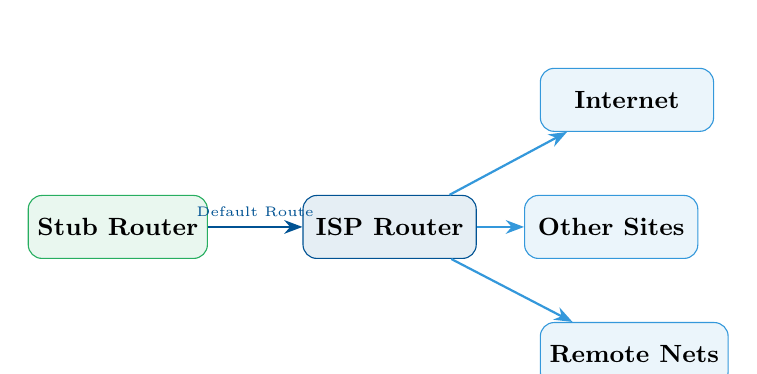
\begin{tikzpicture}[
    node distance=0.5cm,
    box/.style={rectangle, rounded corners=5pt, draw=#1, fill=#1!10, 
               minimum width=2.2cm, minimum height=0.8cm, 
               font=\small\bfseries, align=center},
    arrow/.style={-{Stealth}, thick, #1}
]

% Stub network
\node[box=accent] (stub) {Stub Router};
\node[box=primary, right=1.2cm of stub] (isp) {ISP Router};

\draw[arrow=primary] (stub) -- node[above,font=\tiny] {Default Route} (isp);

% Multiple destinations
\node[box=secondary, above right=0.8cm and 0.8cm of isp] (d1) {Internet};
\node[box=secondary, right=0.6cm of isp] (d2) {Other Sites};
\node[box=secondary, below right=0.8cm and 0.8cm of isp] (d3) {Remote Nets};

\draw[arrow=secondary] (isp) -- (d1);
\draw[arrow=secondary] (isp) -- (d2);
\draw[arrow=secondary] (isp) -- (d3);

\end{tikzpicture}
}
\end{center}

\textbf{Useful When:}
\begin{itemize}
    \item Router has only ONE exit point (stub network)
    \item Single ISP connection
    \item Reduces routing table size significantly
\end{itemize}

\textbf{Dangerous When:}
\begin{itemize}
    \item Multiple exit paths: Default route may blackhole traffic to wrong ISP
    \item Looping: If default route points to router A, and A's default points to B, and B's points to A $\rightarrow$ infinite loop
    \item Backbone routers: Default route on core router can break entire network
\end{itemize}

\textbf{If} you configure default route on R2 (center router), \textbf{but} R2 is backbone, traffic destined for R1's network might loop instead of reaching R1.
\end{abox}

%---

\begin{condbox}
\textbf{Scenario:} You have R1--R2--R3 chain. R1 needs to reach R3's LAN (192.168.3.0/24).

\textbf{Configuration on R1:}
\begin{itemize}
    \item Route 1: \texttt{ip route 192.168.2.0 255.255.255.0 192.168.2.2} (R2's serial interface)
    \item Route 2: \texttt{ip route 192.168.3.0 255.255.255.0 192.168.2.2} (via R2)
\end{itemize}

\textbf{If} you only configure Route 1 to reach R2's network, \textbf{but} forget Route 2 to R3's LAN:
\begin{itemize}
    \item Packets to 192.168.2.x are routed to R2 (OK)
    \item Packets to 192.168.3.x are dropped (no matching route) (FAIL)
\end{itemize}

\textbf{Why R2's Configuration Matters:}
R2 must also have static routes back to R1's LAN and forward to R3's LAN, otherwise return traffic is lost.
\end{condbox}

%---

\begin{whenwhybox}{When is recursive lookup a problem with static routes?}
\textbf{Definition:} Router checks route to reach next-hop, which then checks another route, etc.

\textbf{When It's a Problem:}
\begin{itemize}
    \item \texttt{ip route 192.168.3.0 255.255.255.0 192.168.2.2}
    \item But no connected interface or route to 192.168.2.2
    \item Route marked as invalid
\end{itemize}

\textbf{Prevention:} Always ensure next-hop IP is on a directly connected network or has a route to it.
\end{whenwhybox}

%===============================================================================
\section{Distance-Vector Routing: RIP (Lab 6)}
%===============================================================================

\begin{qbox}{Explain how RIP's distance-vector algorithm works. Why is it called ``distance-vector''?}
\end{qbox}

\begin{abox}
\textbf{``Distance-Vector'' Terminology:}
\begin{itemize}
    \item \textbf{Distance:} Metric (hop count) -- number of routers to destination
    \item \textbf{Vector:} Direction -- next-hop router IP
    \item Example: ``Reach 192.168.3.0 with distance 2 via 192.168.2.2''
\end{itemize}

\textbf{How RIP Works:}

\begin{enumerate}
    \item \textbf{Initial State:} Each router knows only directly connected networks (distance 0)
    
    \item \textbf{Periodic Updates:} Every 30 seconds, send entire routing table to neighbors
    
    \item \textbf{Metric Increase:} Neighbor receives table, increments hop count for each route
    
    \item \textbf{Selection:} Router keeps route with LOWEST hop count
    
    \item \textbf{Convergence:} Over time (30+ seconds), all routers learn all networks
\end{enumerate}

\textbf{Example Convergence:}
\begin{center}
\begin{tabular}{cccc}
\toprule
Time & R1 Knows & R2 Knows & R3 Knows \\
\midrule
0s & Net1(0) & Net2(0) & Net3(0) \\
30s & Net1(0), Net2(1) & Net1(1), Net2(0), Net3(1) & Net2(1), Net3(0) \\
60s & Net1(0), Net2(1), Net3(2) & Net1(1), Net2(0), Net3(1) & Net1(2), Net2(1), Net3(0) \\
\bottomrule
\end{tabular}
\end{center}

\textbf{Limitation:} Hop count doesn't consider bandwidth or delay. A 64kbps serial link with 2 hops might be selected over 1-hop Ethernet!
\end{abox}

%---

\begin{qbox}{What is meant by ``16 hops = unreachable'' in RIP? Why this specific number?}
\end{qbox}

\begin{abox}
\textbf{The 15-Hop Limit:}
\begin{itemize}
    \item Maximum usable distance: 15 hops
    \item 16th hop is unreachable (treated as $\infty$)
    \item This HARD LIMITS network size
\end{itemize}

\textbf{Why 15?}
\begin{itemize}
    \item RIP was designed for networks up to ~50-100 routers max
    \item 15 hops rarely occurs in practice (intended for small networks)
    \item Using 16-bit number: 0xFFFF = 65535 cost, but 16 hops reserved as infinity
\end{itemize}

\textbf{Impact:}
\begin{itemize}
    \item Can never route through more than 15 router hops
    \item Very limiting for large enterprises (100+ routers unreachable)
    \item OSPF has no such limit -- why it's preferred for large networks
\end{itemize}

\textbf{Real-World Implication:} If you have a 20-router chain and RIP on all, routers beyond 15 hops away are unreachable. Network is disconnected!
\end{abox}

%---

\begin{qbox}{Explain RIPv1 vs RIPv2. When would you use each?}
\end{qbox}

\begin{abox}
\begin{center}
\begin{tabularx}{\textwidth}{lXX}
\toprule
\textbf{Feature} & \textbf{RIPv1} & \textbf{RIPv2} \\
\midrule
\textbf{Routing Type} & Classful & Classless \\
\textbf{Subnet Mask} & Assumed, not sent & Sent in updates \\
\textbf{VLSM Support} & No & Yes \\
\textbf{Metric} & Hop count & Hop count (same) \\
\textbf{Update Format} & Broadcast (255.255.255.255) & Multicast (224.0.0.9) \\
\textbf{Convergence} & Slow & Slow (same algorithm) \\
\textbf{MD5 Auth} & No & Yes \\
\textbf{Modern Use} & Rarely & Legacy support \\
\bottomrule
\end{tabularx}
\end{center}

\textbf{When to Use RIPv1:}
\begin{itemize}
    \item Very old equipment (pre-1990s) that only supports RIPv1
    \item Teaching classful routing concepts
    \item Extremely bandwidth-limited networks (v2 slightly larger packets)
\end{itemize}

\textbf{When to Use RIPv2:}
\begin{itemize}
    \item Legacy RIP networks that need VLSM (subnetting)
    \item Migration path to OSPF (still RIP-based but better)
    \item When MD5 authentication required for security
\end{itemize}

\textbf{When to Use Neither:}
\begin{itemize}
    \item Use OSPF if possible (superior in every way for modern networks)
\end{itemize}

\textbf{If} you use RIPv1 with subnets like 192.168.1.0/25 and 192.168.1.128/25, \textbf{then} RIPv1 assumes both are 192.168.1.0/24 and causes routing loops.
\end{abox}

%---

\begin{condbox}
\textbf{Scenario:} You configure RIP on three routers. After 60 seconds, R1 cannot reach R3, although intermediate links are up.

\textbf{Diagnostic Steps:}
\begin{enumerate}
    \item Check \texttt{show ip protocols} -- is RIP enabled?
    \item Verify \texttt{network} statements on all routers (must use CLASSFUL network addresses)
    \item Run \texttt{debug ip rip} to see if updates are being sent
    \item Check \texttt{show ip route} for RIP routes (marked with 'R')
\end{enumerate}

\textbf{Common Causes:}
\begin{itemize}
    \item Forgot to enable RIP on R2 (middle router) -- route never propagates
    \item Used subnet mask instead of classful address in \texttt{network} command
    \item Interface down \textbf{OR} \texttt{no shutdown} missing
    \item Firewall blocking RIP packets (UDP port 520)
\end{itemize}

\textbf{If} convergence is slower than expected (>60 sec), \textbf{but} all routes eventually appear, this is normal. RIP's 30-second update interval + processing time = 60+ seconds.
\end{condbox}

%---

\begin{whenwhybox}{Why does RIP send ENTIRE routing table every 30 seconds?}
\textbf{Reason:} No state tracking -- each router assumes others may have restarted.

\textbf{Consequence:} MASSIVE bandwidth waste!
\begin{itemize}
    \item 100-route network $\times$ 3 routers $\times$ every 30 seconds = continuous traffic
    \item 64kbps serial link becomes choked
    \item WAN administrators hate RIP
\end{itemize}

\textbf{Why Newer Protocols Don't:}
\begin{itemize}
    \item OSPF sends only changes (triggered updates)
    \item Multicast to specific routers (not broadcast to all)
    \item Scales to 10,000+ routes without excessive traffic
\end{itemize}
\end{whenwhybox}

%===============================================================================
\section{Link-State Routing: OSPF (Lab 7)}
%===============================================================================

\begin{qbox}{Explain how OSPF's link-state algorithm differs fundamentally from RIP's distance-vector.}
\end{qbox}

\begin{abox}
\textbf{Fundamental Difference:}

\begin{center}
\begin{tabular}{lcc}
\toprule
& \textbf{Distance-Vector (RIP)} & \textbf{Link-State (OSPF)} \\
\midrule
\textbf{What Each Router Knows} & Only neighbors' routes & Entire network topology \\
\textbf{Algorithm} & Bellman-Ford & Dijkstra SPF \\
\textbf{Metric Source} & Neighbors' reports & Direct link costs \\
\textbf{Loop Prevention} & Split horizon, hold-down & Sequence numbers, aging \\
\bottomrule
\end{tabular}
\end{center}

\textbf{Distance-Vector Analogy:}
\begin{itemize}
    \item Asking neighbor, ``How do I reach network X?''
    \item Neighbor says, ``Go via router Y'' (doesn't explain full path)
    \item You repeat this for each route (like phone game -- info corrupts)
\end{itemize}

\textbf{Link-State Analogy:}
\begin{itemize}
    \item Everyone publishes their own neighborhood map
    \item All routers collect all maps and build complete topology
    \item Each router independently calculates best path to all destinations
    \item Like having GPS with full city map vs. asking locals for directions
\end{itemize}

\textbf{OSPF Process:}

\begin{enumerate}
    \item \textbf{Discover Neighbors:} Hello protocol (every 10 seconds)
    \item \textbf{Exchange Database:} DBD (Database Description) packets
    \item \textbf{Share Link State:} LSA (Link State Advertisements)
    \item \textbf{Build Topology:} Each router has identical topology database
    \item \textbf{Calculate Routes:} Dijkstra SPF algorithm independently
\end{enumerate}

\textbf{Advantage:} All routers calculate simultaneously, preventing inconsistent views.
\end{abox}

%---

\begin{qbox}{What is Router ID (RID) in OSPF, and why must it be stable?}
\end{qbox}

\begin{abox}
\textbf{Router ID:} A 32-bit identifier that uniquely represents an OSPF router in the AS.

\textbf{Selection Precedence:}
\begin{enumerate}
    \item IP explicitly configured with \texttt{router-id} command (highest priority)
    \item Highest IP address of active loopback interfaces
    \item Highest IP address of active physical interfaces (lowest priority)
\end{enumerate}

\textbf{Why Stability Matters:}
\begin{itemize}
    \item RID used in all LSAs as source identifier
    \item RID changes $\rightarrow$ all LSAs are considered from new router
    \item Neighbors think old router died and new router joined
    \item Triggers SPF recalculation (expensive CPU operation)
    \item Repeated RID changes $\rightarrow$ network instability
\end{itemize}

\textbf{Example Problem:}
\begin{itemize}
    \item R1 gets RID = 192.168.1.5 from physical interface (default)
    \item If Fa0/0 goes down, RID changes to 192.168.2.5 (only remaining interface)
    \item All neighbors see RID change as router restart
    \item SPF recalculation triggers (CPU spike)
    \item Network briefly unstable
\end{itemize}

\textbf{Best Practice:} Always configure loopback with stable IP:
\begin{itemize}
    \item \texttt{interface loopback 0}
    \item \texttt{ip address 10.x.x.x 255.255.255.255} (/32 for loopback)
    \item Never goes down (software interface)
    \item Survives any physical interface failure
\end{itemize}
\end{abox}

%---

\begin{qbox}{Explain OSPF cost calculation. Why is it bandwidth-based instead of hop-count?}
\end{qbox}

\begin{abox}
\textbf{OSPF Cost Formula:}
$$\text{Cost} = \frac{10^8}{\text{Bandwidth (bps)}}$$

\textbf{Example Calculations:}
\begin{center}
\begin{tabular}{lll}
\toprule
\textbf{Link Type} & \textbf{Bandwidth} & \textbf{Cost} \\
\midrule
10 Mbps Ethernet & 10,000,000 bps & 10 \\
100 Mbps FastEthernet & 100,000,000 bps & 1 \\
1 Gbps GigabitEthernet & 1,000,000,000 bps & 1 \\
64 kbps Serial & 64,000 bps & 1562 \\
\bottomrule
\end{tabular}
\end{center}

\textbf{Why Bandwidth-Based (Better Than RIP's Hop Count):}

\begin{itemize}
    \item \textbf{Realistic Path Selection:} 1-hop over 64kbps serial avoided in favor of 3-hops over Ethernet
    \item \textbf{Respects Link Quality:} Slow links have higher cost
    \item \textbf{Load Balancing:} Equal-cost paths automatically balanced
\end{itemize}

\textbf{Real-World Comparison:}
\begin{itemize}
    \item RIP: Chooses 1-hop 64kbps serial over 3-hop 1Gbps Ethernet (WRONG!)
    \item OSPF: Chooses 3-hop Ethernet (cost 3) over 1-hop serial (cost 1562) (RIGHT!)
\end{itemize}

\textbf{If} you have slow WAN link and OSPF chooses wrong path, \textbf{then} manually adjust bandwidth:
\begin{itemize}
    \item \texttt{interface serial 0/0/0}
    \item \texttt{bandwidth 128} (set to 128 kbps, not actual 64 kbps)
    \item Cost = 100,000,000 / 128,000 = 781 (still very high, rightfully avoided)
\end{itemize}
\end{abox}

%---

\begin{qbox}{What are OSPF areas, and why would you use them in large networks?}
\end{qbox}

\begin{abox}
\textbf{OSPF Area:} Logical grouping of contiguous networks and routers.

\textbf{Why Areas Exist:}
\begin{itemize}
    \item \textbf{SPF Scalability:} Dijkstra calculation only within area, not entire AS
    \item \textbf{Topology Hiding:} Other areas don't know internal area topology
    \item \textbf{Update Filtering:} Only abstract summary routes cross area boundaries
    \item \textbf{Faster Convergence:} Interior topology change doesn't affect other areas
\end{itemize}

\textbf{OSPF Area Hierarchy:}
\begin{itemize}
    \item \textbf{Area 0 (Backbone):} Required in multi-area OSPF
    \item \textbf{Other Areas:} Must connect to Area 0 (star topology)
    \item Not allowed: Area 1 connects directly to Area 2 (violates design)
\end{itemize}

\textbf{Multi-Area Benefits:}
\begin{center}
\resizebox{0.95\textwidth}{!}{%
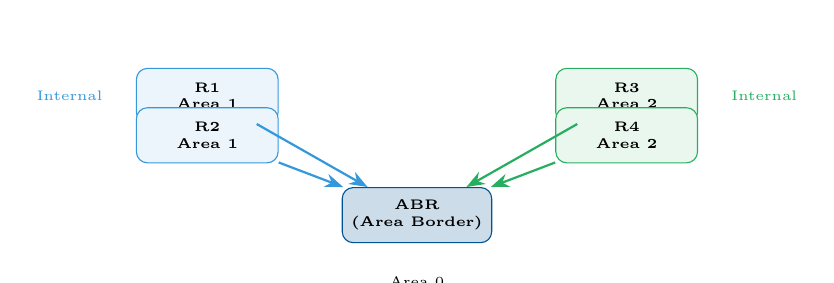
\begin{tikzpicture}[
    node distance=0.6cm,
    box/.style={rectangle, rounded corners=4pt, draw=#1, fill=#1!10, 
               minimum width=1.8cm, minimum height=0.7cm, 
               font=\tiny\bfseries, align=center},
    arrow/.style={-{Stealth}, thick, #1}
]

% Area 0 (backbone)
\node[box=primary, fill=primary!20] (abrtr) {ABR\\(Area Border)};

% Area 1
\node[box=secondary, above left=0.8cm and 0.8cm of abrtr] (r1) {R1\\Area 1};
\node[box=secondary, above left=0.3cm and 0.8cm of abrtr] (r2) {R2\\Area 1};
\draw[arrow=secondary] (r1) -- (abrtr);
\draw[arrow=secondary] (r2) -- (abrtr);

% Area 2
\node[box=accent, above right=0.8cm and 0.8cm of abrtr] (r3) {R3\\Area 2};
\node[box=accent, above right=0.3cm and 0.8cm of abrtr] (r4) {R4\\Area 2};
\draw[arrow=accent] (r3) -- (abrtr);
\draw[arrow=accent] (r4) -- (abrtr);

% Annotations
\node[font=\tiny, below=0.3cm of abrtr] {Area 0};
\node[font=\tiny, left=0.3cm of r1] {\textcolor{secondary}{Internal}};
\node[font=\tiny, right=0.3cm of r3] {\textcolor{accent}{Internal}};

\end{tikzpicture}
}
\end{center}

\textbf{When to Use Multi-Area OSPF:}
\begin{itemize}
    \item Network has $>$ 50-100 routers
    \item Frequent topology changes in one area shouldn't affect others
    \item WAN links need protection from internal area flooding
\end{itemize}

\textbf{When Single-Area is Fine:}
\begin{itemize}
    \item Network $<$ 50 routers (all in Area 0)
    \item Simpler management (no ABR complexity)
    \item Lab environments
\end{itemize}
\end{abox}

%---

\begin{qbox}{Explain the role of Designated Router (DR) and Backup DR in OSPF. When are they elected?}
\end{qbox}

\begin{abox}
\textbf{Why DR/BDR Exist:}

On \textbf{broadcast} networks (like Ethernet), ALL routers would form adjacencies with ALL other routers (meshed topology).
\begin{itemize}
    \item 10 routers = 10 $\times$ 9 / 2 = 45 adjacencies!
    \item Each adjacency sends/receives LSAs (explosion of traffic)
\end{itemize}

\textbf{DR Solution:} Elect one router as central hub.
\begin{itemize}
    \item All routers form adjacencies ONLY with DR and BDR
    \item All routers send updates to DR (multicast 224.0.0.6)
    \item DR floods to all others (multicast 224.0.0.5)
    \item Reduces 45 adjacencies $\rightarrow$ 9 adjacencies (10x improvement)
\end{itemize}

\textbf{DR Election:}
\begin{enumerate}
    \item Router with highest OSPF priority elected (default = 1)
    \item If tie: Router with highest RID elected
    \item Priority 0 = never becomes DR/BDR
\end{enumerate}

\textbf{Example Election:}
\begin{center}
\begin{tabular}{llll}
\toprule
Router & Priority & RID & Result \\
\midrule
R1 & 100 & 10.1.1.1 & \textcolor{highlight}{\textbf{DR}} (highest priority) \\
R2 & 50 & 10.2.2.2 & \textcolor{highlight}{\textbf{BDR}} (2nd highest priority) \\
R3 & 1 & 10.3.3.3 & DROther \\
\bottomrule
\end{tabular}
\end{center}

\textbf{When DR/BDR NOT Needed:}
\begin{itemize}
    \item Point-to-point serial links (only 2 routers, no election)
    \item Frame Relay NBMA networks (special config)
\end{itemize}

\textbf{If} DR fails, \textbf{then} BDR takes over immediately (no re-election needed). If BDR fails first, then new election happens.
\end{abox}

%---

\begin{condbox}
\textbf{Scenario:} You add R4 to existing OSPF network with DR (R1) and BDR (R2). 

\textbf{Question:} Does a new election occur if R4 has highest priority?

\textbf{Answer:} NO! OSPF elects DR/BDR only on first Hello packet exchange. Once elected, they stay until they fail.

\textbf{Why?} Prevents network flapping (constant re-elections). Stability > optimality.

\textbf{If} you want R4 to become DR, \textbf{then} you must:
\begin{enumerate}
    \item Restart OSPF process on the segment (risky, causes outage)
    \item OR change all other routers to priority 0 (R4 now highest)
    \item Better approach: Accept current DR/BDR
\end{enumerate}
\end{condbox}

%---

\begin{whenwhybox}{Why must OSPF Hello and Dead timers match on both sides of a link?}
\textbf{Function:}
\begin{itemize}
    \item Hello Interval: Send Hello packet every N seconds
    \item Dead Interval: If no Hello received in N seconds, neighbor is dead
    \item Default: Hello = 10 sec, Dead = 40 sec (4x Hello)
\end{itemize}

\textbf{If Mismatch:}
\begin{itemize}
    \item R1 expects Hello every 10 sec, has 40-sec dead timer
    \item R2 sends Hello every 20 sec, has 20-sec dead timer
    \item R2 declares R1 dead after 20 sec (before R1 sends next Hello)
    \item Adjacency breaks intermittently
    \item Network becomes unstable
\end{itemize}

\textbf{Best Practice:} Match on all interfaces in a segment. Some defaults:
\begin{itemize}
    \item Ethernet: 10 sec / 40 sec (default)
    \item Serial: 10 sec / 40 sec (same)
    \item Custom: Use \texttt{ip ospf hello-interval} and \texttt{ip ospf dead-interval}
\end{itemize}
\end{whenwhybox}

%===============================================================================
\section{Cross-Lab Comparison \& Advanced Scenarios}
%===============================================================================

\begin{qbox}{If you need to migrate from RIP to OSPF in a live network, what's your strategy?}
\end{qbox}

\begin{abox}
\textbf{Migration Challenge:} Both routing protocols running simultaneously, routing inconsistencies.

\textbf{Strategy:}

\begin{enumerate}
    \item \textbf{Enable OSPF on all routers (don't disable RIP yet):}
    \begin{itemize}
        \item Both protocols run simultaneously
        \item OSPF AD (110) preferred over RIP AD (120)
        \item Traffic prefers OSPF routes
    \end{itemize}

    \item \textbf{Verify OSPF Convergence:}
    \begin{itemize}
        \item Check \texttt{show ip route ospf} -- all networks reachable via OSPF?
        \item Ping critical destinations
        \item Wait 5-10 minutes for full convergence
    \end{itemize}

    \item \textbf{Disable RIP Gradually (site by site, not all at once):}
    \begin{itemize}
        \item Remove RIP from one router
        \item Verify reachability still works (OSPF takes over)
        \item Repeat for each router
    \end{itemize}

    \item \textbf{Remove RIP Configuration:}
    \begin{itemize}
        \item \texttt{no router rip}
        \item \texttt{no network} commands
    \end{itemize}
\end{enumerate}

\textbf{What NOT to Do:}
\begin{itemize}
    \item Disable RIP on all routers simultaneously $\rightarrow$ network black hole if OSPF not ready
    \item Forget to configure OSPF areas $\rightarrow$ topology not following intended structure
\end{itemize}
\end{abox}

%---

\begin{qbox}{When would you use static routing alongside dynamic routing (hybrid approach)?}
\end{qbox}

\begin{abox}
\textbf{Hybrid Scenarios:}

\begin{enumerate}
    \item \textbf{Stub Network with ISP Connection:}
    \begin{itemize}
        \item Internal network: Full OSPF mesh
        \item ISP connection: Static default route
        \item Reason: ISP doesn't participate in our OSPF
    \end{itemize}

    \item \textbf{Security Isolation:}
    \begin{itemize}
        \item OSPF internal network (internal routers)
        \item Static route to DMZ (don't advertise DMZ routes)
        \item Reason: DMZ should be unreachable from internal unless explicitly routed
    \end{itemize}

    \item \textbf{Corporate Acquisition:}
    \begin{itemize}
        \item Company A: OSPF internally
        \item Company B: RIP internally (legacy)
        \item Bridge router: Static routes between them (don't mix protocols)
        \item Reason: Prevents routing loops during integration
    \end{itemize}

    \item \textbf{Bandwidth Management:}
    \begin{itemize}
        \item Expensive WAN link used for static summary route only
        \item OSPF doesn't flood detailed routes over WAN
        \item Reason: Protect expensive link from routing protocol overhead
    \end{itemize}
\end{enumerate}

\textbf{Configuration with Static Default Route:}
\begin{itemize}
    \item \texttt{router ospf 1}
    \item \texttt{network 10.0.0.0 0.0.255.255 area 0}
    \item (Separately) \texttt{ip route 0.0.0.0 0.0.0.0 ISP\_IP}
\end{itemize}

\textbf{If} stub router has BOTH static default route AND OSPF, \textbf{then} OSPF takes precedence for known networks, static route only used for ``everything else''.
\end{abox}

%---

\begin{condbox}
\textbf{Scenario:} You have 4-router network:
\begin{itemize}
    \item R1--R2 (1 Gbps Ethernet, cost = 1)
    \item R2--R3 (64 kbps Serial, cost = 1562)
    \item R3--R4 (1 Gbps Ethernet, cost = 1)
    \item Direct R1--R4 (64 kbps Serial, cost = 1562)
\end{itemize}

\textbf{OSPF Path Selection from R1 to R4:}
\begin{itemize}
    \item Path A: R1$\rightarrow$R2$\rightarrow$R3$\rightarrow$R4 = cost 1 + 1562 + 1 = 1564
    \item Path B: R1$\rightarrow$R4 = cost 1562
    \item \textbf{Result:} R1 chooses Path B (1562 $<$ 1564) (OK) Correct!
\end{itemize}

\textbf{If} serial link R1--R4 has 128 kbps instead, \textbf{then}:
\begin{itemize}
    \item Path B cost = 100,000,000 / 128,000 = 781
    \item Path A cost = still 1564
    \item \textbf{Result:} R1 still chooses Path B (781 $<$ 1564)
\end{itemize}

\textbf{Why This Matters:} Even slightly better bandwidth on a WAN link causes OSPF to prefer it, which might saturate it. Verify paths with \texttt{show ip route} and \texttt{traceroute}.
\end{condbox}

%===============================================================================
\section{Troubleshooting Across All Labs}
%===============================================================================

\begin{qbox}{Interfaces show ``up/down'' instead of ``up/up''. What's the difference, and how do you fix each?}
\end{qbox}

\begin{abox}
\textbf{Interface Status Meanings:}

\begin{center}
\begin{tabularx}{\textwidth}{lXX}
\toprule
\textbf{Status} & \textbf{Physical} & \textbf{Reason \& Fix} \\
\midrule
Up / Up & Both good & Working correctly \\

Up / Down & Physical OK, but Layer 2 issue & \begin{minipage}[t]{\linewidth}
- Missing IP address: \texttt{ip address 10.1.1.1 255.255.255.0}
- Encapsulation mismatch on serial link
- OSPF/RIP not configured on interface
\end{minipage} \\

Down / Down & Physical problem & \begin{minipage}[t]{\linewidth}
- Cable unplugged
- Port shutdown: \texttt{no shutdown}
- Hardware failure
\end{minipage} \\

Administratively Down & Not activated & \texttt{no shutdown} missing \\
\bottomrule
\end{tabularx}
\end{center}

\textbf{Diagnostic Commands:}
\begin{itemize}
    \item \texttt{show ip interface brief} -- Quick status view
    \item \texttt{show ip interface Fa0/0} -- Detailed interface info (includes encapsulation, MTU, ACLs)
    \item \texttt{show running-config interface Fa0/0} -- Check configuration
\end{itemize}
\end{abox}

%---

\begin{qbox}{Routing table shows connected networks but no learned routes. Why?}
\end{qbox}

\begin{abox}
\textbf{Checklist:}

\begin{enumerate}
    \item \textbf{Is routing protocol enabled?}
    \begin{itemize}
        \item \texttt{show ip protocols} -- should show RIP or OSPF
        \item If nothing: Protocol not configured
    \end{itemize}

    \item \textbf{Are network statements correct?}
    \begin{itemize}
        \item RIP: Use classful network addresses (10.0.0.0, 172.16.0.0, etc.)
        \item OSPF: Use specific network + wildcard mask
    \end{itemize}

    \item \textbf{Are interfaces active?}
    \begin{itemize}
        \item \texttt{show ip interface brief} -- all should be Up/Up
        \item If Down: Missing \texttt{no shutdown} or IP address
    \end{itemize}

    \item \textbf{Is neighbor communication working?}
    \begin{itemize}
        \item RIP: Run \texttt{debug ip rip} -- should see periodic updates
        \item OSPF: \texttt{show ip ospf neighbor} -- should see neighbors in FULL state
    \end{itemize}

    \item \textbf{Is there a mismatch in area/process?}
    \begin{itemize}
        \item OSPF: Area ID must match on neighboring routers
        \item RIP: Both routers must have same network statement
    \end{itemize}
\end{enumerate}

\textbf{If} you see neighbors but no routes, \textbf{then} wait 60+ seconds (RIP needs 2 update cycles). If still nothing after 2 minutes, there's likely a configuration error.
\end{abox}

%---

\begin{qbox}{Why would a router show routes in the routing table but packets are still dropped?}
\end{qbox}

\begin{abox}
\textbf{Possible Causes:}

\begin{enumerate}
    \item \textbf{Asymmetric Routing:}
    \begin{itemize}
        \item Forward path: R1$\rightarrow$R2$\rightarrow$R3 (working)
        \item Return path: R3$\rightarrow$different router$\rightarrow$R1 (broken)
        \item Packets arrive at source but never return
        \item Check \texttt{traceroute} in both directions
    \end{itemize}

    \item \textbf{Default Route Problem:}
    \begin{itemize}
        \item Router has route to destination BUT not route back to source
        \item Example: R1 knows how to reach 192.168.3.0, but R3 has no route back to 192.168.1.0
    \end{itemize}

    \item \textbf{Interface Mismatch:}
    \begin{itemize}
        \item Route says ``via 192.168.2.2'' but outgoing interface is configured as 192.168.2.3
        \item Next-hop IP unreachable
    \end{itemize}

    \item \textbf{MTU Mismatch:}
    \begin{itemize}
        \item Packet too large for intermediate link
        \item Dropped silently (ICMP unreachable suppressed)
    \end{itemize}

    \item \textbf{Access Control Lists (ACLs):}
    \begin{itemize}
        \item Route exists but ACL blocks traffic
        \item \texttt{show ip interface} shows ingress/egress ACLs applied
    \end{itemize}
\end{enumerate}

\textbf{Debugging:}
\begin{itemize}
    \item Verify \texttt{show ip route} on source AND destination
    \item Use \texttt{ping} and \texttt{traceroute} from multiple routers
    \item Check \texttt{debug ip routing} to see packet decision process
\end{itemize}
\end{abox}

%---

\begin{condbox}
\textbf{Scenario:} Lab 4 network configured. Pings work between directly connected routers. But PC1 $\rightarrow$ PC3 pings fail.

\textbf{Diagnostic Steps:}
\begin{enumerate}
    \item PC1 can ping its gateway (R1 Fa0/0): (OK) Local link works
    \item R1 can ping R2 S0/0/0: (OK) R1$\rightarrow$R2 link works
    \item R2 can ping R3 S0/0/0: (OK) R2$\rightarrow$R3 link works
    \item R3 can ping PC3: (OK) R3 LAN works
\end{enumerate}

\textbf{But PC1 pings PC3 still fails!}

\textbf{Root Cause:} PC3's default gateway is probably NOT set to R3 Fa0/0.

\textbf{Fix:} Set PC3 gateway to R3's LAN IP.

\textbf{If} gateway is set but pings still fail, \textbf{then}:
\begin{itemize}
    \item Check reverse route on R3: does it know how to reach 192.168.1.0?
    \item Check clock rate on R2 serial interface (DCE side)
    \item Run \texttt{show ip route} on all three routers -- verify all networks present
\end{itemize}
\end{condbox}

%===============================================================================
\section{Viva Quick Reference}
%===============================================================================

\subsection{Key Definitions}

\begin{description}
    \item[Administrative Distance (AD):] Trustworthiness of route source. Lower = more trusted. Static=1, OSPF=110, RIP=120.
    
    \item[Convergence:] Time for all routers to learn all routes. RIP=30+ sec, OSPF=immediate.
    
    \item[Hop Count:] Number of router hops to destination. RIP metric.
    
    \item[Cost (OSPF):] Bandwidth-based metric. $\text{Cost} = 10^8 / \text{Bandwidth}$.
    
    \item[LSA (Link State Advertisement):] OSPF packet containing link state information.
    
    \item[Hello Protocol:] OSPF neighbor discovery. Default every 10 seconds.
    
    \item[Router ID (RID):] Unique 32-bit identifier for OSPF router. Configured or auto-assigned from highest IP.
    
    \item[Designated Router (DR):] OSPF elected router on broadcast networks to minimize adjacencies.
    
    \item[Wildcard Mask:] Inverse of subnet mask. Used in OSPF network statements.
\end{description}

%===============================================================================
\section{Final Exam Strategy}
%===============================================================================

\subsection{Common Viva Questions Pattern}

\begin{enumerate}
    \item \textbf{Explain \ldots} (Conceptual)
    \begin{itemize}
        \item Answer: Definition + why important + how used
        \item Include: Advantages AND limitations
    \end{itemize}

    \item \textbf{Compare \ldots} (Cross-evaluation)
    \begin{itemize}
        \item Use table format
        \item Always mention when to use each
        \item Give real-world example
    \end{itemize}

    \item \textbf{What if \ldots} (Conditional)
    \begin{itemize}
        \item State the problem clearly
        \item Explain why it happens
        \item Describe solution
        \item Mention prevention/best practice
    \end{itemize}

    \item \textbf{Design a network with \ldots} (Application)
    \begin{itemize}
        \item Draw topology
        \item Choose appropriate routing protocol
        \item Justify your choice
        \item Mention potential issues
    \end{itemize}
\end{enumerate}

\subsection{Must-Know Distinctions}

\begin{itemize}
    \item Static vs Dynamic: Manual vs Automatic
    \item Distance-Vector vs Link-State: Neighbor reports vs Full topology
    \item RIP vs OSPF: Hop count vs Bandwidth-based cost
    \item RIPv1 vs RIPv2: Classful vs Classless routing
    \item DCE vs DTE: Clock provider vs Clock receiver
    \item Single-Area vs Multi-Area OSPF: Simplicity vs Scalability
    \item DR/BDR: Only on broadcast networks, not point-to-point
\end{itemize}

\end{document}
